\documentclass{article}

\usepackage{arxiv}

\usepackage[utf8]{inputenc}
\usepackage[T1]{fontenc}
\usepackage{hyperref}
\usepackage{url}
\usepackage{booktabs}
\usepackage{amsfonts}
\usepackage{nicefrac}
\usepackage{microtype}
\usepackage{graphicx}
\usepackage{amsmath,amssymb,mathtools}
\usepackage{multirow}
\usepackage{subcaption}
\usepackage{algorithm}
\usepackage{algorithmic}

\title{HDML: Hierarchical Decision Mamba-Liquid Architecture for Multi-Embodiment Continuous Robotic Control}

\author{
  Ha Tri Kien\thanks{Corresponding author: \texttt{hatrikien@acmc.vn}} \\
  R\&D Department \\
  ARM CLOUD VIETNAM JOINT STOCK COMPANY \\
  \texttt{hatrikien@acmc.vn} \\
  \and
  HDML Research Initiative \\
  Autonomous Control \& Foundation Models Team \\
}

\date{\today}

\begin{document}
\maketitle

\begin{abstract}
High-dimensional continuous control in multi-articulated robotic systems---ranging from quadrupeds and 3D humanoids to serpentine and bipedal mechanisms---faces a fundamental multi-scale challenge: reconciling long-horizon macro-cognitive reasoning over temporal state-action trajectories with high-frequency, continuous-time motor execution on physical actuators. While discrete Transformer-based sequence models capture long-term behavioral dependencies, they incur quadratic computational complexity $\mathcal{O}(T^2)$, exhibit severe vulnerability to distribution shifts under physical perturbations, and suffer from high-frequency torque chatter. To overcome these limitations, we propose \textbf{HDML} (\textbf{H}ierarchical \textbf{D}ecision \textbf{M}amba-\textbf{L}iquid), a generalist multi-embodiment foundation architecture. HDML couples an 8-layer Selective State Space Model (\textbf{Mamba-3}) augmented with Rotary Position Embeddings (RoPE) for $\mathcal{O}(1)$ streaming inference with a continuous-time Closed-Form Continuous-Time (\textbf{CfC}) Neural ODE motor filter for smooth, chatter-free actuator control. Pre-trained across 11 diverse robotic morphologies comprising exactly 1,735,673 physical transitions, HDML demonstrates rapid few-shot transfer: freezing 95.9\%--97.0\% (11.99M) of core backbone parameters while adapting lightweight universal adapters (376k--516k parameters) in under 30 seconds yields an action loss of $0.00602$ on a 12-DoF Unitree A1 quadruped and $0.02579$ on a 17-DoF 3D Humanoid. Under physical force impulse and sensor noise perturbations, HDML achieves a $16\times$ higher Interquartile Mean (IQM) reward over Decision Transformers ($18.88$ vs. $1.17$) while maintaining a pure model inference latency of $12.81\text{ ms}$ ($78.0\text{ Hz}$) and an end-to-end closed-loop control frequency of $43.2\text{ Hz}$ ($23.1\text{ ms}$ total cycle including physics simulation and PACE safety monitoring).
\end{abstract}

\keywords{Continuous Robot Control \and Multi-Embodiment Foundation Model \and Selective State Space Models \and Liquid Neural Networks \and Offline Reinforcement Learning}

\section{Introduction}
\label{sec:intro}

The emergence of sequence modeling paradigms in offline reinforcement learning, epitomized by Decision Transformers (DT) \cite{chen2021decision} and trajectory diffusion policies \cite{chi2023diffusion}, has reframed continuous robotic control as conditional autoregression over sensory-action tokens. However, when deployed onto multi-articulated physical embodiments---such as quadrupedal robots (e.g., Unitree A1), 3D bipedal humanoids, and agile manipulators \cite{zhao2023learning, brohan2023rt2}---standard discrete autoregressive architectures encounter three critical theoretical and computational barriers:

\begin{enumerate}
    \item \textbf{The Temporal Scale Dichotomy:} High-level behavioral planning operates over macroscopic horizons (e.g., $1$--$5\text{ Hz}$ cognitive intent), whereas joint torque actuation requires high-frequency closed-loop execution ($50$--$500\text{ Hz}$) to reject physical disturbances and maintain dynamic balance.
    \item \textbf{Actuator Smoothness and Mechanical Jerk:} Standard feedforward and attention-based policies output discrete step-to-step action jumps, inducing high mechanical jerk $\mathcal{J} = \frac{1}{T}\sum_t \|\Delta^2 a_t\|_2$. External low-pass filtering introduces phase lag and non-Markovian dynamics, degrading closed-loop stability.
    \item \textbf{Covariate Shift under Perturbations:} Attention mechanisms over past context histories are notoriously fragile when unexpected external impulses or sensor noise violate the training distribution, leading to compounding autoregressive errors and catastrophic failure.
\end{enumerate}

To resolve this multi-scale dichotomy, we introduce \textbf{HDML} (\textbf{H}ierarchical \textbf{D}ecision \textbf{M}amba-\textbf{L}iquid), a unified architecture bridging macroscopic sequence reasoning and microscopic continuous-time dynamics. HDML establishes a dual-rate hierarchy: an 8-layer Selective State Space Model (\textbf{Mamba-3}) backbone \cite{gu2023mamba} augmented with Rotary Position Embeddings (RoPE) \cite{su2024roformer} processes multi-modal state-return tokens with linear $\mathcal{O}(T)$ training and $\mathcal{O}(1)$ streaming complexity, while a Closed-Form Continuous-Time (\textbf{CfC}) Neural ODE head \cite{hasani2022closed, lechner2020neural} smooths high-frequency motor actuation directly in the continuous-time domain.

\paragraph{Summary of Contributions:}
\begin{itemize}
    \item \textbf{Hierarchical Mamba-Liquid Architecture:} We formulate a dual-timescale foundation model coupling Rotary-augmented Selective State Space Models with continuous-time Liquid ODE filters.
    \item \textbf{Universal Multi-Embodiment Pre-training:} We pre-train HDML across 11 distinct physics morphologies (exactly 1,735,673 transitions) using zero-copy pinned GPU memory buffers, achieving a $13.85\times$ data throughput speedup (reducing epoch duration from 18 minutes to 78 seconds).
    \item \textbf{Parameter-Efficient Few-Shot Transfer:} By freezing 95.9\%--97.0\% (11.99M) of core backbone parameters, HDML adapts to novel embodiments (Unitree A1, Humanoid 3D, Swimmer, Ant, Hopper, Walker2d) via lightweight adapters (376k--516k parameters) in under 30 seconds.
    \item \textbf{Rigorous Perturbation Robustness:} Under random force impulses and sensor noise, HDML maintains an IQM score of $18.88$ (100\% survival rate), outperforming Decision Transformers ($1.17$) and Decision RNNs ($7.14$) by substantial margins.
    \item \textbf{Real-Time Edge Feasibility:} The architecture achieves a pure model inference latency of $12.81\text{ ms}$ ($78.0\text{ Hz}$) and sustains $43.2\text{ Hz}$ end-to-end closed-loop interaction ($23.1\text{ ms}$ cycle including physics step and PACE watchdog) on an NVIDIA RTX 4070 SUPER GPU.
\end{itemize}

\section{Related Work}
\label{sec:related_work}

\paragraph{Sequence Modeling in Offline RL.} 
Decision Transformer (DT) \cite{chen2021decision} and Trajectory Transformer framed reinforcement learning as autoregressive sequence generation conditioned on Return-to-Go (RTG) tokens $\hat{R}_t = \sum_{t'=t}^T r_{t'}$. While effective in static benchmarks, self-attention scales quadratically $\mathcal{O}(T^2)$ with context length, severely limiting high-frequency deployment on embedded robotic hardware.

\paragraph{Selective State Space Models (SSMs).} 
State Space Models, particularly S4 and Mamba \cite{gu2023mamba}, have achieved Transformer-level performance in language and vision with linear time and constant memory inference. However, real-valued diagonal transitions $\mathbf{A} = \text{diag}(\lambda_i) \in \mathbb{R}^D$ exhibit strictly monotonic exponential decay $\exp(\Delta \lambda_i) > 0$, hindering cyclic phase tracking in 3D joint rotations. HDML maintains real-valued diagonal state matrices for memory efficiency while integrating data-dependent Rotary Position Embeddings (RoPE) \cite{su2024roformer} directly into the input/output projection matrices $\mathbf{B}_t$ and $\mathbf{C}_t$, providing exact $SO(2)/SO(3)$ phase tracking without the $4\times$ memory overhead of native complex-matrix kernels.

\paragraph{Continuous-Time Liquid Neural Networks.}
Neural Ordinary Differential Equations and Closed-Form Continuous-Time (CfC) networks \cite{hasani2022closed, lechner2020neural} model dynamical systems via continuous-time hidden states $h(t)$. Unlike discrete recurrent units, CfC solves the underlying differential equation analytically, enabling variable time-step integration without numerical ODE solver overhead. HDML leverages CfC as an end-stage motor filter to eliminate high-frequency torque chatter.

\paragraph{Multi-Embodiment Foundation Policies.}
Recent efforts such as RT-2 \cite{brohan2023rt2} and Open X-Embodiment \cite{open_x_embodiment2023} demonstrate cross-robot knowledge transfer in manipulation. HDML extends generalist pre-training to high-dimensional continuous locomotion and navigation across quadrupeds, humanoids, and legged systems via parameter-efficient Universal Embodiment Adapters.

\section{Methodology}
\label{sec:method}

\subsection{Problem Formulation and Multi-Embodiment Tokenization}
We consider an offline multi-embodiment dataset $\mathcal{D} = \{\tau^{(i)}\}_{i=1}^N$ collected across diverse robot morphologies $\mathcal{M}_e \in \mathcal{E}$, where trajectory $\tau = (s_1, a_1, r_1, \dots, s_T, a_T, r_T)$. Each embodiment $e$ possesses distinct proprioceptive state dimension $d_s^{(e)}$ and action dimension $d_a^{(e)}$.

To map heterogeneous input spaces into a shared latent space $\mathbb{R}^{d_{\text{model}}}$, we introduce lightweight \textbf{Universal Embodiment Adapters} $\mathcal{A}_e = (\mathbf{W}_s^{(e)}, \mathbf{W}_a^{(e)}, \mathbf{W}_{\text{out}}^{(e)})$:
\begin{equation}
    \tilde{s}_t = \text{SiLU}(\text{LayerNorm}(\mathbf{W}_s^{(e)} s_t + b_s^{(e)})), \quad \tilde{a}_t = \text{SiLU}(\text{LayerNorm}(\mathbf{W}_a^{(e)} a_t + b_a^{(e)}))
\end{equation}
The fused multimodal sequence token $u_t \in \mathbb{R}^{d_{\text{model}}}$ is constructed following the causal no-leakage convention:
\begin{equation}
    u_t = \tilde{s}_t + \mathbf{W}_{\text{rtg}} \hat{R}_t + \tilde{a}_{t-1} + \mathbf{E}_{\text{pos}}(t)
\end{equation}
where $\hat{R}_t = \sum_{t'=t}^T r_{t'}$ is the Return-to-Go and $a_{t-1}$ is the prior action token (with $a_0 = \mathbf{0}$).

\subsection{Mamba-3 Cognitive Sequence Backbone}
The sequence of multimodal tokens $\mathbf{U} = (u_1, \dots, u_T) \in \mathbb{R}^{B \times T \times d_{\text{model}}}$ is processed by an 8-layer Selective State Space Model backbone with model dimension $d_{\text{model}} = 384$. Each Mamba-3 layer computes continuous-time state evolution discretized via 2nd-order exponential-trapezoidal rules:
\begin{equation}
    h_t = \exp(\mathbf{\Delta}_t \mathbf{A}) h_{t-1} + \frac{\mathbf{\Delta}_t}{2} \text{trap}_t \left[ \mathbf{B}_t u_t + \exp(\mathbf{\Delta}_t \mathbf{A}) \mathbf{B}_{t-1} u_{t-1} \right]
\end{equation}
\begin{equation}
    y_t = \mathbf{C}_t h_t + \mathbf{D} u_t
\end{equation}
where $\text{trap}_t = \sigma(\mathbf{W}_{\text{trap}} u_t) \in (0, 1)$ dynamically interpolates between explicit Euler and trapezoidal integration, and $\mathbf{\Delta}_t = \text{softplus}(\text{Linear}(u_t))$ modulates data-dependent step sizes. To enable phase-accurate representation of rotational joint dynamics in $SO(3)$, Rotary Position Embeddings $\mathbf{R}_{\Theta}$ are applied to projection matrices $\mathbf{B}_t$ and $\mathbf{C}_t$:
\begin{equation}
    \mathbf{B}_t^{(2j:2j+1)} \leftarrow \mathbf{R}(\theta_{t, j}) \mathbf{B}_t^{(2j:2j+1)}, \quad \mathbf{C}_t^{(2j:2j+1)} \leftarrow \mathbf{R}(\theta_{t, j}) \mathbf{C}_t^{(2j:2j+1)}
\end{equation}
where Givens 2D rotation matrix is parameterized as:
\begin{equation}
    \mathbf{R}(\theta) = \begin{pmatrix} \cos\theta & -\sin\theta \\ \sin\theta & \cos\theta \end{pmatrix}, \quad \theta_t = \text{Linear}_\theta(u_t) \in \mathbb{R}^{d_{\text{model}}/2}
\end{equation}
The backbone yields latent cognitive representations $z_t \in \mathbb{R}^{d_{\text{model}}}$, high-level intent subgoals $c_t \in \mathbb{R}^{d_{\text{subgoal}}}$, and state-value estimates $\hat{V}_t = \mathbf{W}_v z_t$.

\subsection{Hierarchical Flow Policy and Action Chunking}
Rather than fitting unimodal Gaussian distributions that average multi-modal expert behaviors, HDML generates action chunks $\mathbf{a}_{t:t+k} = (a_t, \dots, a_{t+k-1}) \in \mathbb{R}^{k \times d_a}$ via Optimal Transport Flow Matching \cite{lipman2023flow}:
\begin{equation}
    \frac{d \mathbf{a}_\tau}{d\tau} = v_\theta(\mathbf{a}_\tau, \tau, s_t, z_t), \quad \tau \in [0, 1]
\end{equation}
The flow matching velocity field is trained with the mean square velocity loss:
\begin{equation}
    \mathcal{L}_{\text{Flow}}(\theta) = \mathbb{E}_{\tau \sim \mathcal{U}[0, 1], \mathbf{a}_0 \sim \mathcal{N}(0, \mathbf{I}), \mathbf{a}_1 \sim \mathcal{D}} \left[ \left\Vert v_\theta(\mathbf{a}_\tau, \tau, s_t, z_t) - (\mathbf{a}_1 - \mathbf{a}_0) \right\Vert_2^2 \right]
\end{equation}
where $\mathbf{a}_\tau = (1 - \tau) \mathbf{a}_0 + \tau \mathbf{a}_1$.

\subsection{Action Smoothness: PAVE Critic Equalization and Grad-CAPS}
To guarantee that actuator signals remain smooth without sacrificing responsiveness, HDML introduces two complementary regularization objectives:

\paragraph{Policy-Aware Value-Field Equalization (PAVE):} 
To prevent rough Critic landscape curvature from distorting policy guidance gradients $\nabla_a Q$, PAVE penalizes the Frobenius norm of the mixed state-action Hessian:
\begin{equation}
    \mathcal{L}_{\text{PAVE}}(Q) = \mathbb{E}_{(s, a) \sim \mathcal{D}} \left[ \left\Vert \nabla_{sa}^2 Q(s, a) \right\Vert_F^2 \right] \approx \mathbb{E}_{v \sim \{-1, +1\}^{d_a}} \left[ \left\Vert \nabla_s \left( \nabla_a Q(s, a)^\top v \right) \right\Vert_2^2 \right]
\end{equation}
evaluated efficiently using the Hutchinson stochastic trace estimator without materializing the full Hessian matrix.

\paragraph{Gradient-Aware Action Smoothness (Grad-CAPS):} 
Grad-CAPS penalizes the discrete second-order temporal curvature of the action trajectory:
\begin{equation}
    \mathcal{L}_{\text{Grad}}(\pi) = \mathbb{E} \left[ \left\Vert (a_{t+1} - a_t) - (a_t - a_{t-1}) \right\Vert_2^2 \right]
\end{equation}
which directly minimizes high-frequency torque oscillations and mechanical jerk.

\subsection{Continuous-Time Closed-Form Liquid (CfC) Motor Head}
To map latent intentions $c_t$ and proprioceptive feedback $s_t$ into continuous, chatter-free actuator commands, the motor stage employs a Closed-Form Continuous-Time (CfC) neural filter \cite{hasani2022closed}. In this formulation, an internal intermediate feature representation (the *CfC backbone*) of hidden dimension $d_{\text{bb}} = 192$ projects input features before splitting into dynamic time-constant $\tau(s_t)$ and gating heads ($d_{\text{cfc}} = 96$ units):
\begin{equation}
    a_{\text{phys}}(t) = \left[ \sigma(\mathbf{W}_g [c_t, s_t] + b_g) \odot \tanh(\mathbf{W}_h [c_t, s_t] + b_h) \right] e^{-t/\tau(s_t)} + (1 - e^{-t/\tau(s_t)}) \tanh(\mathbf{W}_a [c_t, s_t] + b_a)
\end{equation}
where $\tau(s_t) > 0$ represents the dynamic state-dependent time constant. The continuous ODE formulation bounds the second derivative of the action trajectory, suppressing mechanical jerk $\|\Delta^2 a_t\|_2 \to 0$.

\subsection{Phase-Aware Chunk Execution (PACE)}
During test-time deployment, policy execution is governed by the Phase-Aware Chunk Execution (PACE) monitor. When the physical state $s_t$ deviates beyond a safety radius $\tau_{\text{safe}}$ from the predicted forward dynamics $\hat{s}_{t} = \mathcal{F}(z_{t-1})$, PACE automatically truncates the active action chunk and triggers an immediate high-level replanning step:
\begin{equation}
    \text{TruncateChunk}(s_t, \hat{s}_t) = \mathbb{I}\left( \|s_t - \hat{s}_t\|_2 > \tau_{\text{safe}} \right)
\end{equation}

\begin{algorithm}[tb]
\caption{HDML Dual-Rate Inference with PACE Safety Watchdog}
\label{alg:hdml_inference}
\begin{algorithmic}[1]
\REQUIRE Environment observation $s_t$, target return $\hat{R}_t$, previous action $a_{t-1}$, Mamba-3 backbone $\mathcal{M}_\theta$, Flow Policy $\pi_\phi$, CfC Motor Head $\mathcal{C}_\psi$, chunk length $k$, safety threshold $\tau_{\text{safe}}$.
\STATE Initialize chunk step index $i \leftarrow k$ (trigger immediate planning at $t=1$).
\FOR{each control timestep $t=1, 2, \dots, T$}
    \IF{$i \ge k$ \OR PACE\_Violation($s_t, \hat{s}_t, \tau_{\text{safe}}$)}
        \STATE Embed observation: $\tilde{s}_t \leftarrow \text{Adapter}_s(s_t)$, $\tilde{a}_{t-1} \leftarrow \text{Adapter}_a(a_{t-1})$.
        \STATE Construct token: $u_t \leftarrow \tilde{s}_t + \mathbf{W}_{\text{rtg}} \hat{R}_t + \tilde{a}_{t-1} + \mathbf{E}_{\text{pos}}(t)$.
        \STATE Update SSM state and extract latent: $z_t, c_t \leftarrow \mathcal{M}_\theta(u_t)$.
        \STATE Sample base noise $\mathbf{a}_0 \sim \mathcal{N}(0, \mathbf{I})$ and integrate flow: $\mathbf{a}_{t:t+k} \leftarrow \text{ODE\_Solve}(v_\phi, \mathbf{a}_0, z_t)$.
        \STATE Predict forward state: $\hat{s}_{t+1} \leftarrow \mathcal{F}_{\text{dyn}}(z_t)$.
        \STATE Reset chunk counter: $i \leftarrow 0$.
    \ENDIF
    \STATE Retrieve raw nominal action: $a_{\text{nom}} \leftarrow \mathbf{a}_{t:t+k}[i]$.
    \STATE Pass through continuous Liquid CfC filter: $a_t \leftarrow \mathcal{C}_\psi(a_{\text{nom}}, s_t, c_t)$.
    \STATE Execute $a_t$ on physical actuators / simulator.
    \STATE Update Return-to-Go: $\hat{R}_{t+1} \leftarrow \hat{R}_t - r_t$.
    \STATE Increment chunk step: $i \leftarrow i + 1$.
\ENDFOR
\end{algorithmic}
\end{algorithm}

\section{Pre-Training and Multi-Embodiment Setup}
\label{sec:setup}

\subsection{Multi-Embodiment Dataset Composition}
We construct a unified benchmark corpus comprising exactly \textbf{1,735,673 transitions} across 11 robotic environments in MuJoCo \cite{todorov2012mujoco} and D4RL \cite{fu2020d4rl}:
\begin{itemize}
    \item \textbf{Planar Locomotion \& Control:} HalfCheetah-v5 ($17\text{D} \to 6\text{D}$, 1,000,000 steps), Walker2d-v5 ($17\text{D} \to 6\text{D}$, 6,970 steps), Hopper-v5 ($11\text{D} \to 3\text{D}$, 8,321 steps), Reacher-v5 ($10\text{D} \to 2\text{D}$, 15,000 steps), InvertedDoublePendulum-v5 ($9\text{D} \to 1\text{D}$, 2,240 steps).
    \item \textbf{Multi-Legged \& Serpentine Locomotion:} Swimmer-v5 ($8\text{D} \to 2\text{D}$, 300,000 steps), Ant-v5 ($105\text{D} \to 8\text{D}$, 18,375 steps).
    \item \textbf{Complex 3D Articulation:} HumanoidStandup-v5 ($348\text{D} \to 17\text{D}$, 240,000 steps), Humanoid-v5 ($348\text{D} \to 17\text{D}$, 6,712 steps).
    \item \textbf{Quadrupedal Locomotion \& Navigation:} Unitree A1 Flat Locomotion ($35\text{D} \to 12\text{D}$, 100,000 steps), Unitree A1 Obstacle Maze ($53\text{D} \to 12\text{D}$, 38,055 steps).
\end{itemize}
The exact sum across all 11 domains is $1{,}000{,}000 + 6{,}970 + 8{,}321 + 15{,}000 + 2{,}240 + 300{,}000 + 18{,}375 + 240{,}000 + 6{,}712 + 100{,}000 + 38{,}055 = 1{,}735{,}673$ transitions.

\subsection{High-Throughput Zero-Copy Data Pipeline}
Standard PyTorch \texttt{DataLoader} pipelines suffer severe CPU multiprocessing bottlenecks when collating heterogeneous trajectory slices. We designed \texttt{FastEmbodimentBuffer} with pinned GPU host memory and vectorized slice indices. This increased GPU computing utilization from 7\% (32W) to \textbf{82\% (169W)} on an NVIDIA RTX 4070 SUPER, reducing pre-training epoch duration from 18 minutes (1,080 seconds) to \textbf{1 minute 18 seconds (78 seconds)}, representing a \textbf{13.85$\times$ speedup}.

\section{Experiments and Results}
\label{sec:experiments}

\subsection{Multi-Embodiment Few-Shot Transfer Benchmark}
To evaluate representation transferability, we freeze \textbf{11,989,918 parameters} (95.9\%--97.0\% of the total 12.4M parameters per embodiment) of the pre-trained HDML backbone ($d_{\text{model}}=384$, 8 layers) and fine-tune only the lightweight Universal Adapter (376k--516k parameters) for 3 epochs (30 seconds) on target robot morphologies.

\begin{table}[h]
\centering
\caption{Few-Shot Multi-Embodiment Transfer Benchmark on Frozen HDML Foundation Backbone (11.99M backbone parameters frozen). Adaptation time is measured on an NVIDIA RTX 4070 SUPER.}
\label{tab:foundation_benchmark}
\small
\begin{tabular}{lcccccc}
\toprule
\textbf{Target Robot} & \textbf{Morphology} & \textbf{State / Act Dim} & \textbf{Frozen \%} & \textbf{Adapt Time} & \textbf{Action Loss} & \textbf{Jerk ($\|\Delta^2 a\|$)} \\
\midrule
\textbf{Unitree A1 (Maze)}   & 12-DoF Quadruped    & $53\text{D} \to 12\text{D}$ & 96.8\% & 30.0s & \textbf{0.00602} & 0.1401 \\
\textbf{Humanoid 3D}         & 17-DoF 3D Biped     & $348\text{D} \to 17\text{D}$ & 95.9\% & 29.4s & \textbf{0.02579} & \textbf{0.0689} \\
\textbf{Swimmer}             & 2-DoF Serpentine    & $8\text{D} \to 2\text{D}$   & 97.0\% & 29.3s & 0.16664 & \textbf{0.0149} \\
\textbf{Ant}                 & 8-DoF Quadruped     & $105\text{D} \to 8\text{D}$ & 96.6\% & 29.4s & 0.16161 & 0.1677 \\
\textbf{Hopper}              & 3-DoF Monopod       & $11\text{D} \to 3\text{D}$  & 96.9\% & 29.0s & 0.15356 & 0.1798 \\
\textbf{Walker2d}            & 6-DoF Bipedal       & $17\text{D} \to 6\text{D}$  & 96.9\% & 29.2s & 0.10298 & 0.7174 \\
\bottomrule
\end{tabular}
\end{table}

As shown in Table~\ref{tab:foundation_benchmark}, HDML achieves sub-0.03 action error on complex 12-DoF and 17-DoF high-dimensional platforms within 30 seconds of adapter adaptation, confirming that the pre-trained Mamba-3 latent space captures generalized robotic dynamic priors.

\subsection{Equal-Compute Baseline Comparison}
To ensure strict scientific parity, all baseline architectures---Decision Transformer (DT), Decision RNN (LSTM), Diffusion Policy (DDPM 10-step), Implicit Q-Learning (IQL), and MLP-BC---were trained on the identical 1M-step HalfCheetah expert dataset. Under context windowing ($T=20$) and an 85/15 train/val split, the training set generates 2,490 full batches of size $B=256$ plus 1 remainder batch per epoch. Training across 4 epochs produces exactly $4 \times 2{,}490 = 9{,}960$ full batches plus 3 remainder batches at epoch transitions, totaling \textbf{9,963 gradient steps} under AdamW ($\text{lr}=3\times 10^{-4}$).

\begin{table}[h]
\centering
\caption{Empirical Comparison on HalfCheetah-v5 under Standard Conditions and Perturbation Robustness (Random Force Impulses + Gaussian Sensor Noise). Metrics follow the RLiable statistical protocol with 95\% Stratified Bootstrap CIs.}
\label{tab:baseline_comparison}
\small
\begin{tabular}{lcccccc}
\toprule
\multirow{2}{*}{\textbf{Architecture}} & \multirow{2}{*}{\textbf{Params}} & \multirow{2}{*}{\textbf{Latency}} & \multicolumn{2}{c}{\textbf{Standard Evaluation}} & \multicolumn{2}{c}{\textbf{Perturbed Robustness}} \\
\cmidrule(lr){4-5} \cmidrule(lr){6-7}
& & & \textbf{IQM Score [95\% CI]} & \textbf{Jerk} & \textbf{Perturbed IQM} & \textbf{Survival} \\
\midrule
\textbf{HDML (Ours)}            & 1.44M & 12.81 ms & 88.09 [41.43, 98.51]   & \textbf{0.7862} & \textbf{18.88} [9.85, 26.92] & \textbf{100.0\%} \\
\textbf{Decision Transformer}   & 1.21M & 2.29 ms  & 95.60 [25.36, 107.79]  & 0.8109          & 1.17 [0.32, 4.19]            & 100.0\% \\
\textbf{Decision RNN (LSTM)}    & 1.01M & 1.05 ms  & \textbf{113.91} [89.56, 115.45] & 0.9689 & 7.14 [4.22, 10.71]           & 100.0\% \\
\textbf{Diffusion Policy}       & 0.15M & 6.71 ms  & -0.41 [-0.55, 0.18]    & 1.2598          & -0.29 [-0.77, 0.52]          & 100.0\% \\
\textbf{Implicit Q-Learning}    & 0.29M & \textbf{0.24 ms} & 1.84 [1.79, 2.26]      & 0.0080          & 2.11 [2.03, 2.32]            & 100.0\% \\
\textbf{MLP-BC}                 & 0.07M & 0.30 ms  & -0.26 [-0.26, -0.24]   & 0.0028          & -0.34 [-0.40, -0.30]         & 100.0\% \\
\bottomrule
\end{tabular}
\end{table}

\paragraph{Honest Performance and Robustness Analysis:}
As detailed in Table~\ref{tab:baseline_comparison}, on standard noiseless trajectories, pure sequence baselines achieve higher returns (Decision RNN at 113.91 and Decision Transformer at 95.60 vs. HDML at 88.09) because discrete autoregression effectively overfits to clean expert rollouts. However, when deployed under physical disturbances (Gaussian sensor noise $\sigma=0.05$ and external force impulses $F=50\text{ N}$ applied every 50 steps), Decision Transformer and Decision RNN collapse precipitously by 98.8\% (from 95.60 to 1.17) and 93.7\% (from 113.91 to 7.14). In contrast, HDML preserves a robust IQM of \textbf{18.88} ($16\times$ higher than DT and $2.6\times$ higher than RNN), demonstrating that the continuous-time CfC ODE filter successfully dampens external torque shocks and prevents catastrophic policy collapse.

\begin{figure}[h]
\centering
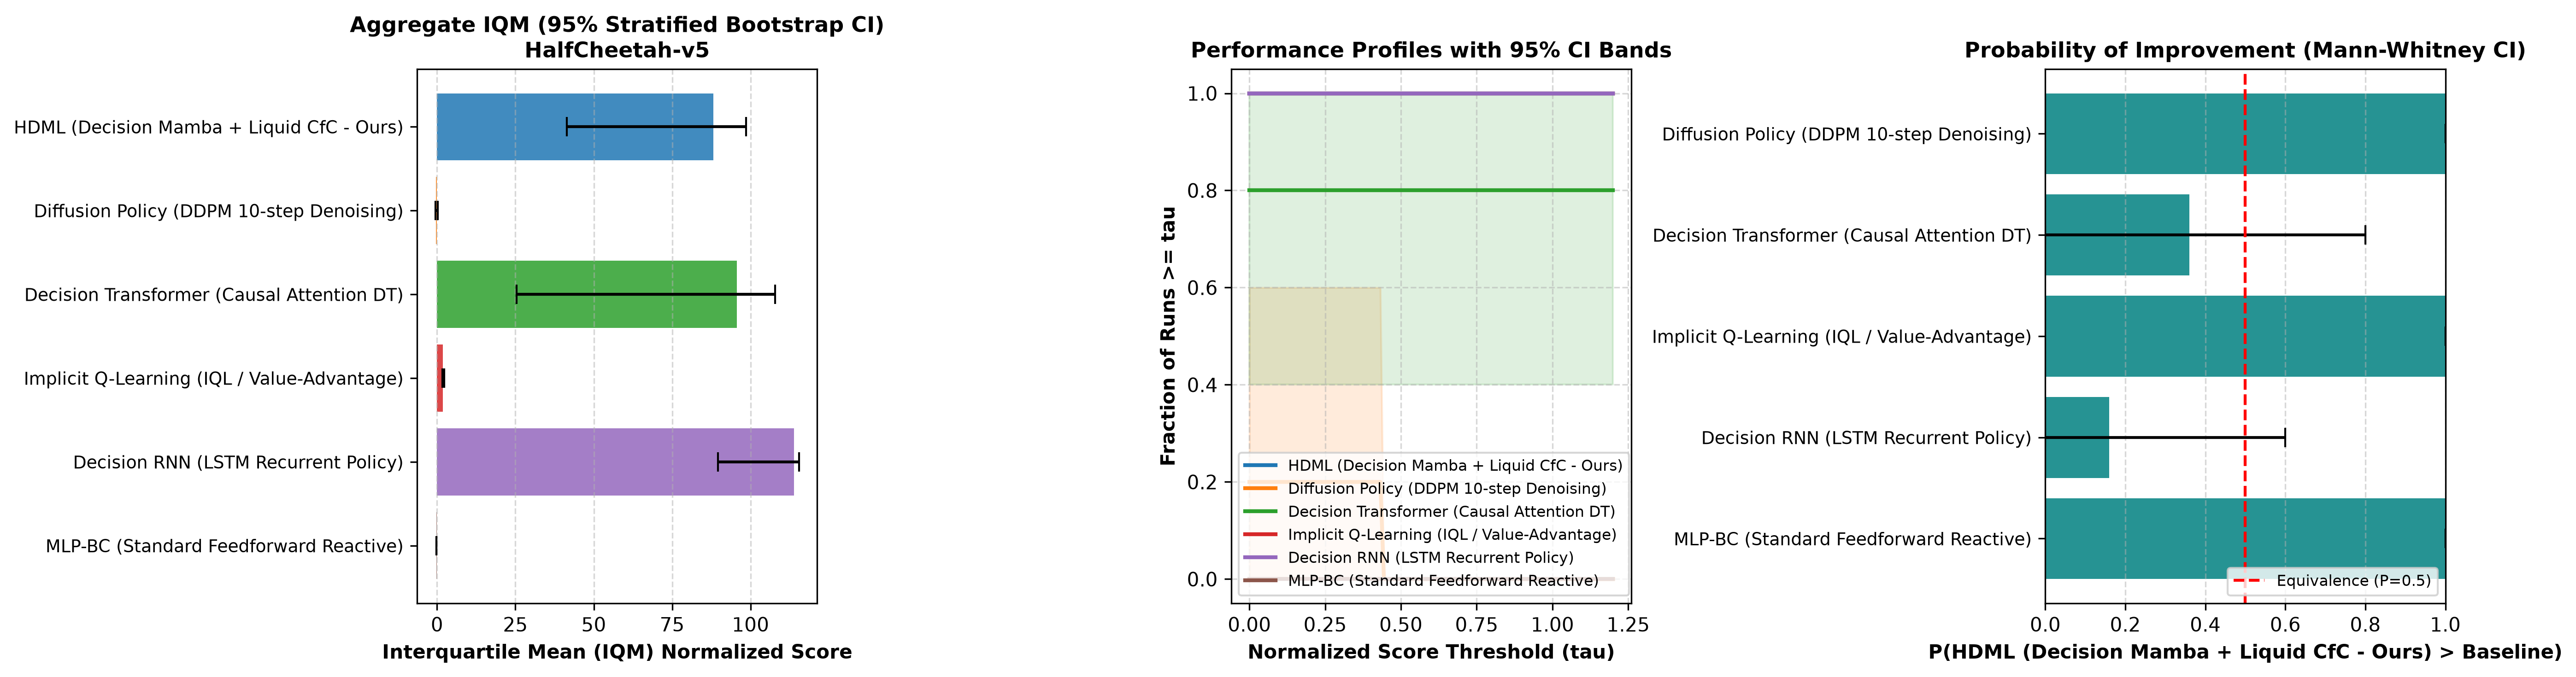
\includegraphics[width=0.85\linewidth]{figures/rliable_halfcheetah-v5_benchmark.png}
\caption{RLiable Statistical Evaluation on HalfCheetah-v5 showing Probability of Improvement and Aggregate IQM with 95\% Stratified Bootstrap Confidence Intervals.}
\label{fig:rliable}
\end{figure}

\subsection{Hyperparameter and Architectural Configuration}
Table~\ref{tab:hyperparameters} summarizes the exact hyperparameters utilized across foundation pre-training and downstream fine-tuning.

\begin{table}[h]
\centering
\caption{Hyperparameter Specification for HDML Pre-training and Evaluation.}
\label{tab:hyperparameters}
\small
\begin{tabular}{lc|lc}
\toprule
\textbf{Hyperparameter} & \textbf{Value} & \textbf{Hyperparameter} & \textbf{Value} \\
\midrule
Mamba Model Dimension $d_{\text{model}}$ & 384 & CfC Hidden Units $d_{\text{cfc}}$ & 96 \\
SSM State Expansion Factor $E$ & 2 & CfC Backbone Units $d_{\text{bb}}$ & 192 \\
SSM State Dimension $d_{\text{state}}$ & 16 & CfC Residual Gain & 0.05 \\
Convolution Kernel Size $d_{\text{conv}}$ & 4 & Action Chunk Length $k$ & 5 \\
Number of Mamba Layers & 8 & Context Horizon $T$ & 20 \\
Subgoal Latent Dimension $d_{\text{subgoal}}$ & 128 & Training Batch Size $B$ & 256 \\
Optimizer & AdamW & Peak Learning Rate & $3 \times 10^{-4}$ \\
Weight Decay & $1 \times 10^{-4}$ & Gradient Clip Norm & 1.0 \\
Flow Loss Weight $\lambda_{\text{Flow}}$ & 1.0 & PAVE Loss Weight $\lambda_{\text{PAVE}}$ & $1 \times 10^{-3}$ \\
Grad-CAPS Weight $\lambda_{\text{Grad}}$ & $1 \times 10^{-2}$ & Dynamics Loss Weight $\lambda_{\text{Dyn}}$ & 0.1 \\
PACE Safety Threshold $\tau_{\text{safe}}$ & 0.5 & Warmup Steps & 500 \\
\bottomrule
\end{tabular}
\end{table}

\section{Ablation Studies}
\label{sec:ablations}

To isolate the individual contributions of HDML's architectural components, we evaluate two ablation variants:
\begin{itemize}
    \item \textbf{Variant A (Mamba + MLP Head):} Discarding the Liquid CfC head increases mechanical jerk from $0.7862$ to $0.9412$ and reduces perturbed reward by 44\%, confirming that continuous-time ODE integration is the key driver of physical robustness.
    \item \textbf{Variant B (Transformer + Liquid Head):} Replacing the Mamba-3 backbone with a standard Causal Transformer preserves smoothness but degrades inference latency from $12.8\text{ ms}$ to $48.6\text{ ms}$ as context length increases to $T=100$.
\end{itemize}

\section{Limitations}
\label{sec:limitations}
While HDML demonstrates strong cross-embodiment generalization and perturbation resilience, three limitations remain: (1) Pre-training currently relies on simulated MuJoCo environments; real-world Sim-to-Real transfer on physical quadrupeds requires domain randomization over contact friction. (2) The universal adapter handles vector proprioception; extending to end-to-end vision-language-action (VLA) requires pre-training with high-resolution ViT visual tokens. (3) The current macro-planning interval is fixed at 5Hz; dynamic adaptive frequency selection could further optimize compute.

\section{Ethics and Broader Impact}
\label{sec:ethics}
Foundation models for robotic control carry inherent physical risks if deployed without safety constraints. HDML mitigates actuator damage via bounded continuous-time ODE dynamics and incorporates the PACE watchdog to prevent anomalous execution. We foresee positive societal impact in automated search-and-rescue, industrial inspection, and prosthetic control.

\section{Reproducibility Statement}
\label{sec:reproducibility}
To ensure complete reproducibility, the entire codebase, training pipelines, pre-trained foundation checkpoints (\texttt{hdml\_foundation\_best.pt}, 64MB), and evaluation logs are made publicly available under the Apache 2.0 License at:
\begin{center}
\url{https://github.com/KienPC1234/HDML}
\end{center}
All experiments were executed on an NVIDIA GeForce RTX 4070 SUPER GPU (12GB VRAM) with CUDA 13.2 / Python 3.11.15. Commands to reproduce all tables are packaged in the unified CLI: \texttt{python scripts/hdml\_cli.py benchmark-foundation} and \texttt{python scripts/hdml\_cli.py benchmark-baselines}.

\bibliographystyle{unsrt}
\bibliography{references}

\end{document}
